\begin{myposter}{
    Глава 2. Смена ролика в контакте с опорной плоскостью
}

    \headerbox
    {Уравнения движения вырождаются на стыках роликов}
    {name=first,column=0,row=0,span=3}
    {
        {\huge\bf
            \vspace{10pt}
            Разрыв 2ого рода в правой части из-за выражений $(l\cos\chi_i-r)$ в знаменателе.\\
            Исключим достижение острия ролика, усекая ролики и допуская пересечение их тел.
            \begin{figure}[H]
                \centering
                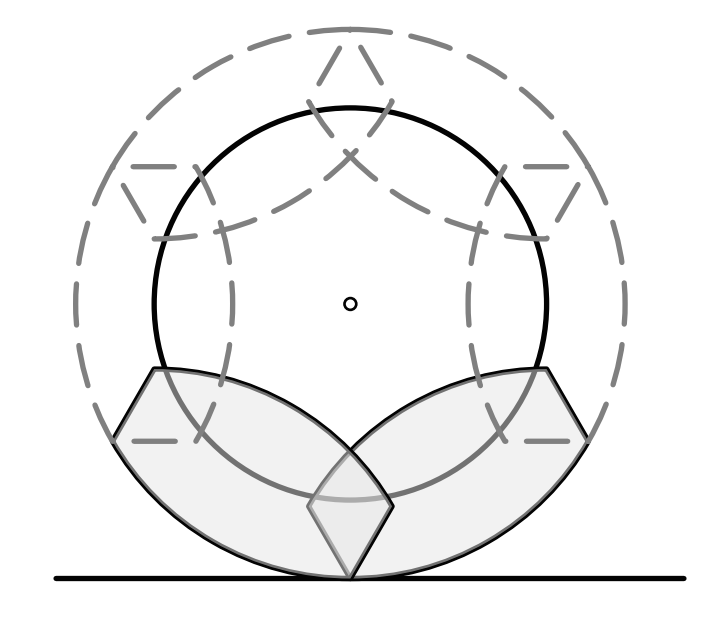
\includegraphics[width=0.5\textwidth]{content/pic/asypng/pic_overlap.png}
                % \asyinclude{content/pic/asy/pic_overlap.asy}
                % \caption{Ролики перекрываются}
            \end{figure}
            \vspace{10pt}
        }
    }
    
    \headerbox
    {Ролики входят и выходят из состояния контакта при $t = t^*$}
    {name=second,column=0,row=1,below=first,span=3}
    {
        {\huge\bf
            \vspace{10pt}
            Происходит мгновенное снятие связи с одного ролика и наложение связи на другой.\\
            Пусть:
            \begin{itemize}
                \item $\Delta t << 1$, $\quad \Delta \q \sim \dotq\Delta t << 1$, $\quad \Delta \dotq < \infty$,
                \item к моменту окончания удара $t^*+\Delta t$ уравнения связей выполнены (\enspace $\dqposle = \cstr(\q)\nuposle \ $)
                \item верно основное уравнение удара \enspace $\eqDeltaqQ$
                \item связи идеальны \enspace $\Q^T\delta\qposle = 0$, где $\delta\qposle$ -- виртуальные перемещения, допустимые вновь наложенными связями
            \end{itemize}
            \vspace{10pt}
        }
    }

\end{myposter}
